\documentclass[a4 paper]{article}
% Set target color model to RGB
\usepackage[inner=2.0cm,outer=2.0cm,top=2.5cm,bottom=2.5cm]{geometry}
\usepackage{setspace}
\usepackage[rgb]{xcolor}
\usepackage{verbatim}
\usepackage{subcaption}
\usepackage{amsgen,amsmath,amstext,amsbsy,amsopn,tikz,amssymb,tkz-linknodes}
\usepackage{fancyhdr}
\usepackage[colorlinks=true, urlcolor=blue,  linkcolor=blue, citecolor=blue]{hyperref}
\usepackage[colorinlistoftodos]{todonotes}
\usepackage{rotating}
\usepackage{hyperref}
%\usetikzlibrary{through,backgrounds}
\hypersetup{%
pdfauthor={Ashudeep Singh},%
pdftitle={Assignment 4},%
pdfkeywords={Tikz,latex,bootstrap,uncertaintes},%
pdfcreator={PDFLaTeX},%
pdfproducer={PDFLaTeX},%
}
%\usetikzlibrary{shadows}
% \usepackage[francais]{babel}
\usepackage{booktabs}
\newcommand{\ra}[1]{\renewcommand{\arraystretch}{#1}}

\newtheorem{thm}{Theorem}[section]
\newtheorem{prop}[thm]{Proposition}
\newtheorem{lem}[thm]{Lemma}
\newtheorem{cor}[thm]{Corollary}
\newtheorem{defn}[thm]{Definition}
\newtheorem{rem}[thm]{Remark}
\numberwithin{equation}{section}

\newcommand{\homework}[6]{
   \pagestyle{myheadings}
   \thispagestyle{plain}
   \newpage
   \setcounter{page}{1}
   \noindent
   \begin{center}
   \framebox{
      \vbox{\vspace{2mm}
    \hbox to 6.28in { {\bf COMP 3005:~Database Management Systems \hfill {\small (#2)}} }
       \vspace{6mm}
       \hbox to 6.28in { {\Large \hfill #1  \hfill} }
       \vspace{6mm}
       \hbox to 6.28in { {\it Instructor: {\rm #3} \hfill Name: {\rm #5}, ID: {\rm #6}} }
       %\hbox to 6.28in { {\it TA: #4  \hfill #6}}
      \vspace{2mm}}
   }
   \end{center}
   \markboth{#5 -- #1}{#5 -- #1}
   \vspace*{4mm}
}

\newcommand{\problem}[2]{~\\\fbox{\textbf{Q #1}}\hfill (#2 points)\newline\newline}
\newcommand{\subproblem}[1]{~\newline\textbf{(#1)}}
\newcommand{\D}{\mathcal{D}}
\newcommand{\Hy}{\mathcal{H}}
\newcommand{\VS}{\textrm{VS}}
\newcommand{\solution}{~\newline\textbf{\textit{(Solution)}} }

\newcommand{\bbF}{\mathbb{F}}
\newcommand{\bbX}{\mathbb{X}}
\newcommand{\bI}{\mathbf{I}}
\newcommand{\bX}{\mathbf{X}}
\newcommand{\bY}{\mathbf{Y}}
\newcommand{\bepsilon}{\boldsymbol{\epsilon}}
\newcommand{\balpha}{\boldsymbol{\alpha}}
\newcommand{\bbeta}{\boldsymbol{\beta}}
\newcommand{\0}{\mathbf{0}}



\begin{document}
\homework{Look Inna Book}{Due: Friday Apr. 3, 2020 (11:59 PM)}{Ahmed El-Roby}{}{Devon Hope}{101038344}

\tableofcontents
\newpage
\section{Conceptual Design}
\qquad This section explains and demonstrates how the database uses the ER-Diagram to store and hold all neccessary information given in the project summary. 
\subsection{ER-Diagram}
{\centering 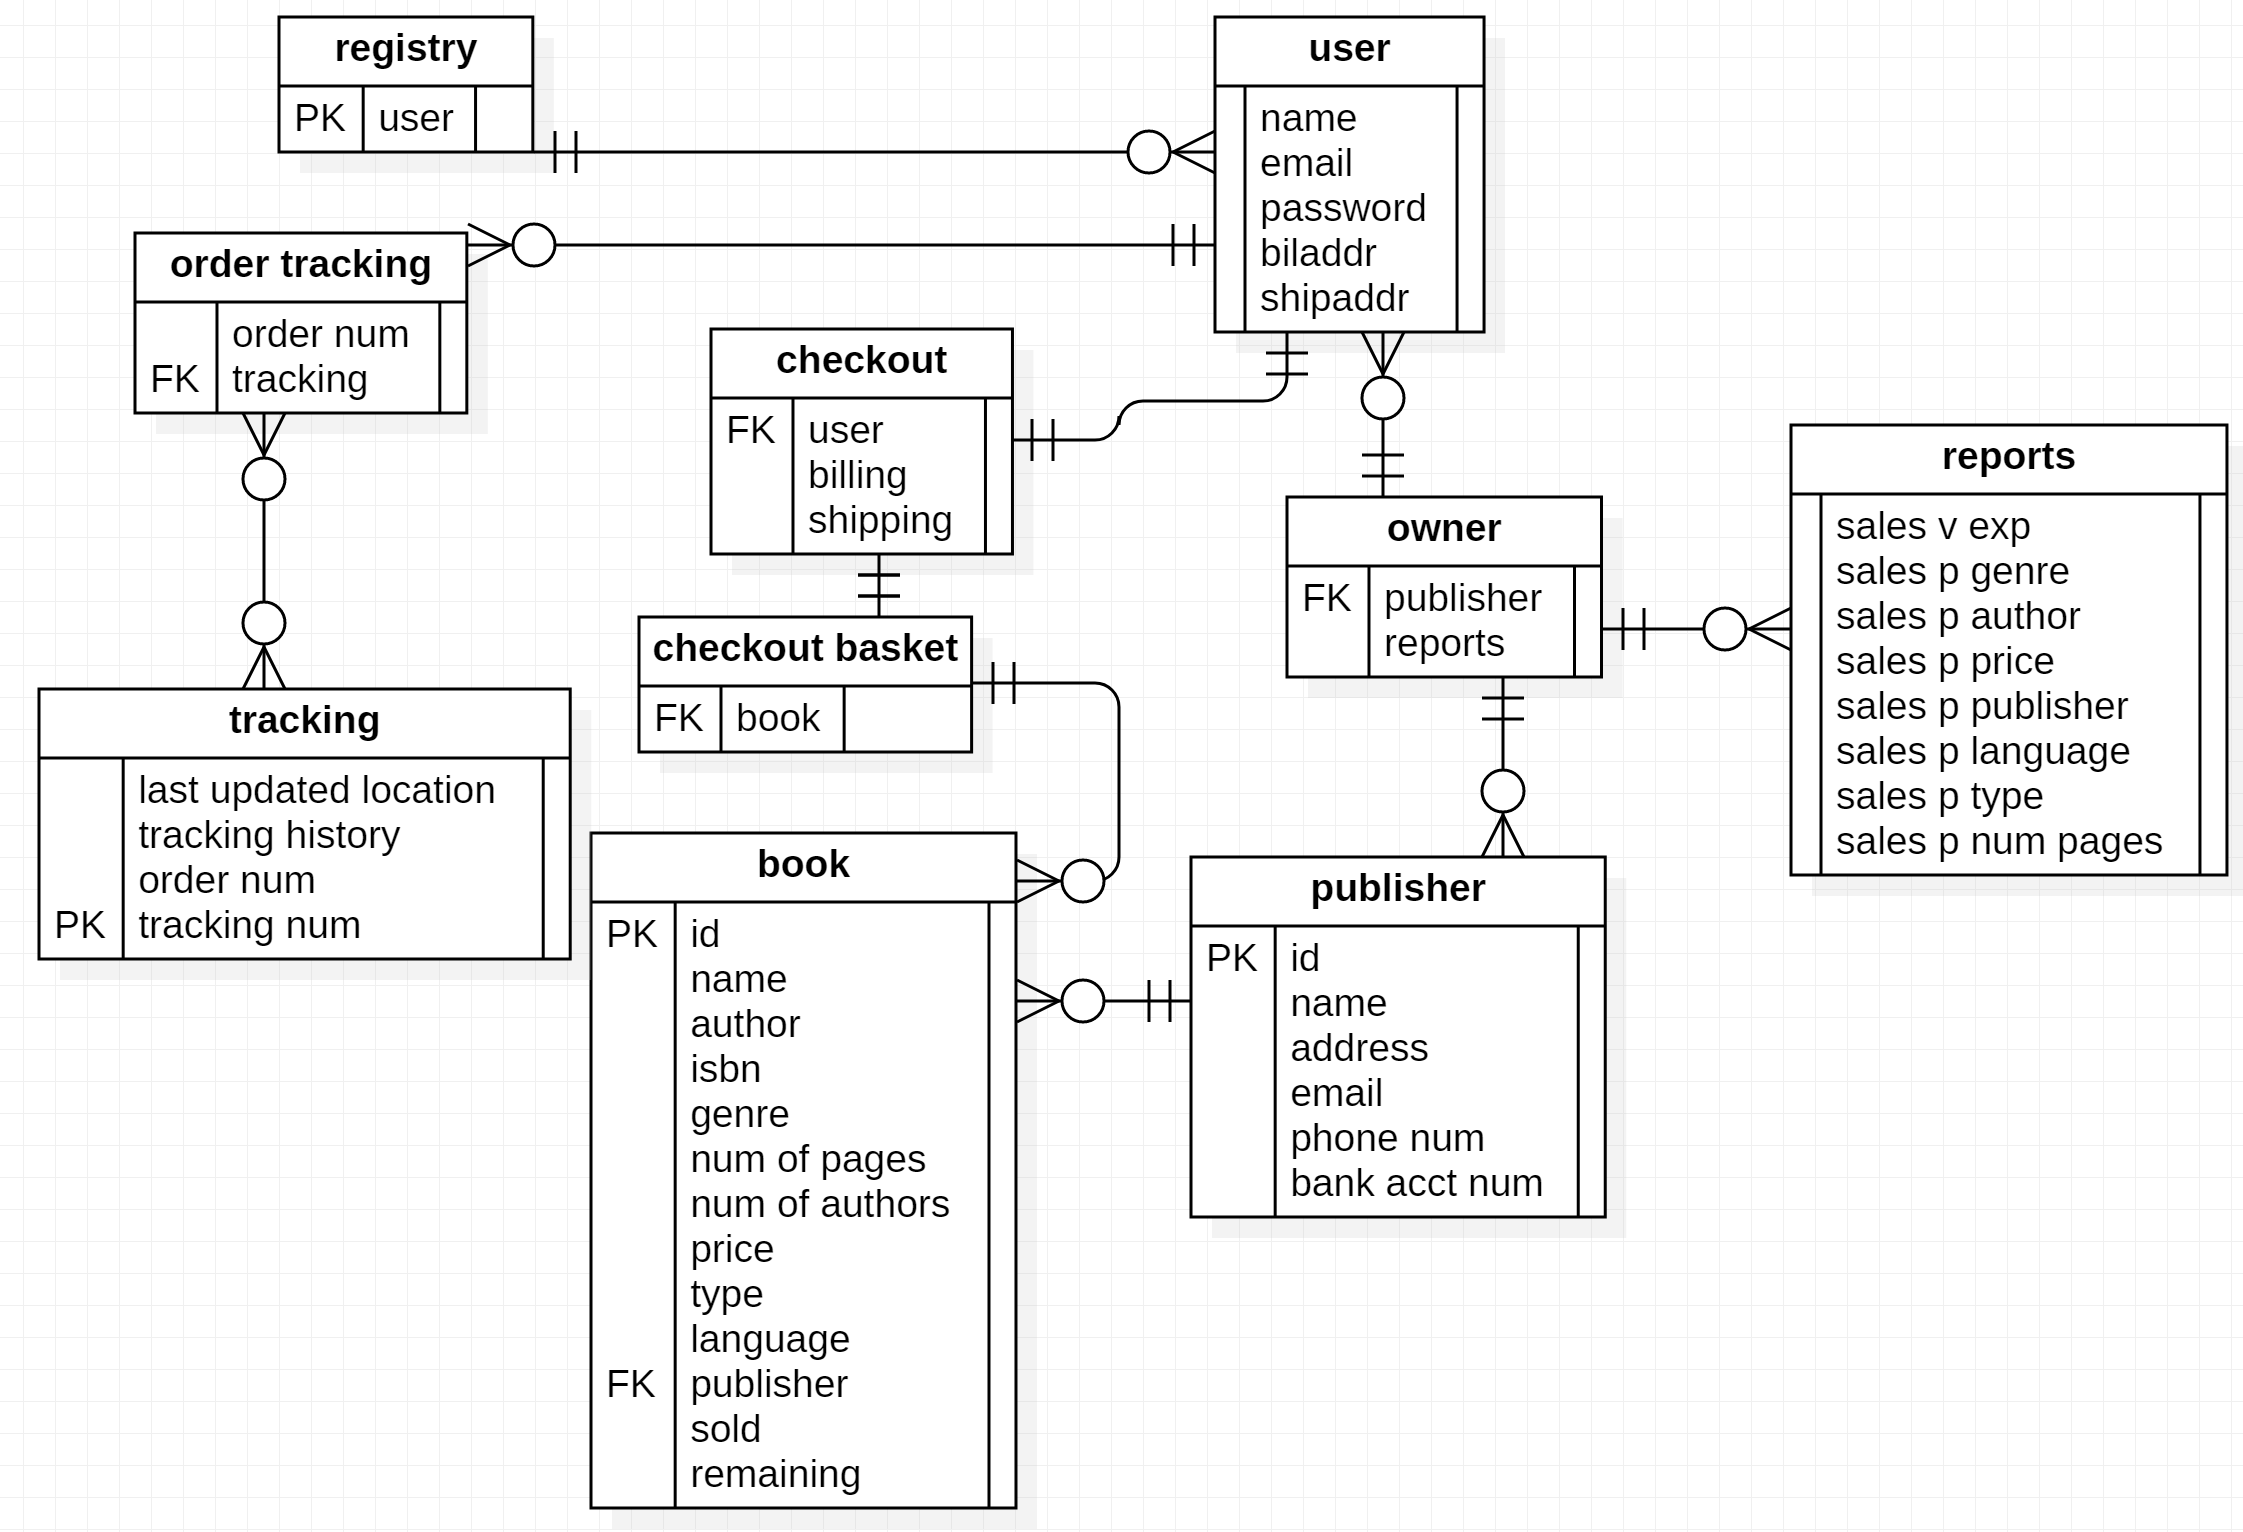
\includegraphics[width=\textwidth/1]{ER_D.png}}
\subsection{Explanation}
\qquad This diagram contains all of the necessary entities to store all necessary information created by and used by the user in the program during runtime. All user information is stored in the user entity when they are signed into the program, this way everything they need is easily accessible. All of the users cart and checkout information is stored in the entities checkout and checkout basket, checkout stores the user id, records their shipping and billing addresses, and checkout basket stores all of the books in the users cart, the book entity is a foreign key for the book entity. When the user goes to checkout their cart, and is successful, all tracking information for their order is stored in the order tracking entity and the final tracking information from the third party shipping company is given and stored in the tracking entity. The tracking entity is a foreign key for the order tracking entity. The publisher entity holds all information needed by the user and the owner of the store on each publisher, the user only needs a name whereas the owner can see all other information required. The owner entity holds all of the relevant information for the owner, such as the a foreign key for the publisher entity id. The reports entity holds all of the reports created by the program. 
\section{Reduction to Relation Schemas}
\section{Normalization of Relation Schemas}
\section{Database Schema Diagram}
\section{Implementation}
\subsection{Overview}
\subsection{Scenarios}
\section{Github Repostiory}
\href{https://github.com/WalterMitty2112/Online-Bookstore-Webapp}{Look Inna Book: Online Bookstore}
\section{Instructions for Submission}


\end{document}